\documentclass[11pt,a4paper,oneside]{article}

\usepackage [utf8x] {inputenc}
\usepackage [T2A] {fontenc}

\usepackage{fancybox}
\usepackage{fancyhdr}
\usepackage{lastpage}

\usepackage{setspace}
\usepackage{colortbl}
\usepackage[warn]{mathtext}

\usepackage[labelsep=period]{caption}

\usepackage{xcolor}
\usepackage{hyperref}
\usepackage{graphicx}

\usepackage{amsmath}

\graphicspath{{picks/}}

\usepackage[shortlabels]{enumitem}
\usepackage{array}
\usepackage{ifthen}
\usepackage{pdfpages}
\usepackage[strict]{changepage}

\usepackage{tikz}
\usetikzlibrary{calc}
\usetikzlibrary{decorations.pathmorphing}

\newcolumntype{P}[1]{>{\centering\arraybackslash}p{#1}}

\usepackage[left=12mm, top=12mm, right=12mm, bottom=28mm, nohead, footskip=10mm]{geometry} % настройки полей документа 20 15 15 35

\newcommand{\sect}[2] {
    \addtocounter{section}{1}
    \section*{\Huge\thesection.\,#1}
    \addcontentsline{toc}{subsection}{ \texorpdfstring{\thesection.\qquad\qquad #2}{Lg}}
}

\newcommand{\subsec}[2] {
    \addtocounter{subsection}{1}
    \subsection*{\thesubsection.\,#1}
    \addcontentsline{toc}{subsection}{ \texorpdfstring{\quad \thesubsection.\qquad\ #2}{Lg}}
}

\newcommand{\subsubsec}[2] {
    \addtocounter{subsubsection}{1}
    \subsubsection*{\thesubsubsection.\,#1}
    \addcontentsline{toc}{subsection}{ \texorpdfstring{\quad\quad\ \thesubsubsection. #2}{Lg}}
}


\newcommand{\labnum}{
    1.2.2
}

\fancypagestyle{plain}{ %
	\fancyhf{} % remove everything
	\renewcommand{\headrulewidth}{0pt} % lines
	\renewcommand{\footrulewidth}{0pt}
	
	\fancyfoot[L]{\ifthenelse{\isodd{\thepage}}{Работа \labnum}{\thepage}}
	
	\fancyfoot[R]{\ifthenelse{\isodd{\thepage}}{\thepage}{Работа \labnum}}
}

\pagestyle{plain}

\begin{document}
	\setcounter{tocdepth}{4}
	\setcounter{section}{0}
	\setcounter{subsection}{0}
	\setcounter{subsubsection}{0}
	\textheight = 240mm
	\footskip = 10mm
    
    { % add title page
        \leftskip = 25mm
    	{\white{.}} \\[0.2cm]

\Title{\bf{\huge
\begin{center}
{Работа \labnum }
\end{center}}} \\[0.4 cm]

{\bf{\Large
\begin{center}
{\noindent ЭКСПЕРИМЕНТАЛЬНАЯ ПРОВЕРКА ЗАКОНА\\ ВРАЩАТЕЛЬНОГО ДВИЖЕНИЯ НА\\ КРЕСТООБРАЗНОМ МАЯТНИКЕ}
\end{center}}} \\[0.1cm]

{\begin{center}\Large{Работу выполнил Матренин Василий Б01-006 \\[0.8cm]}\end{center}}

{\bf{\noindent Цель работы: }}  экспериментально проверить уравнение (1), получив зависимость\\ углового ускорения от момента инерции и момента прикладываемых к системе сил,\\ а также проанализировать влияние сил трения, действующих в оси вращения. \\[0.4cm]

{\bf{\noindent В работе используются: }} Крестообразный маятник Обербека; компьютер \\[0.4cm]

\newpage
        \leftskip = 10mm
    }
    
    \begin{center}
    \Large{\bf Схема установки:}
\end{center}

\begin{center}
    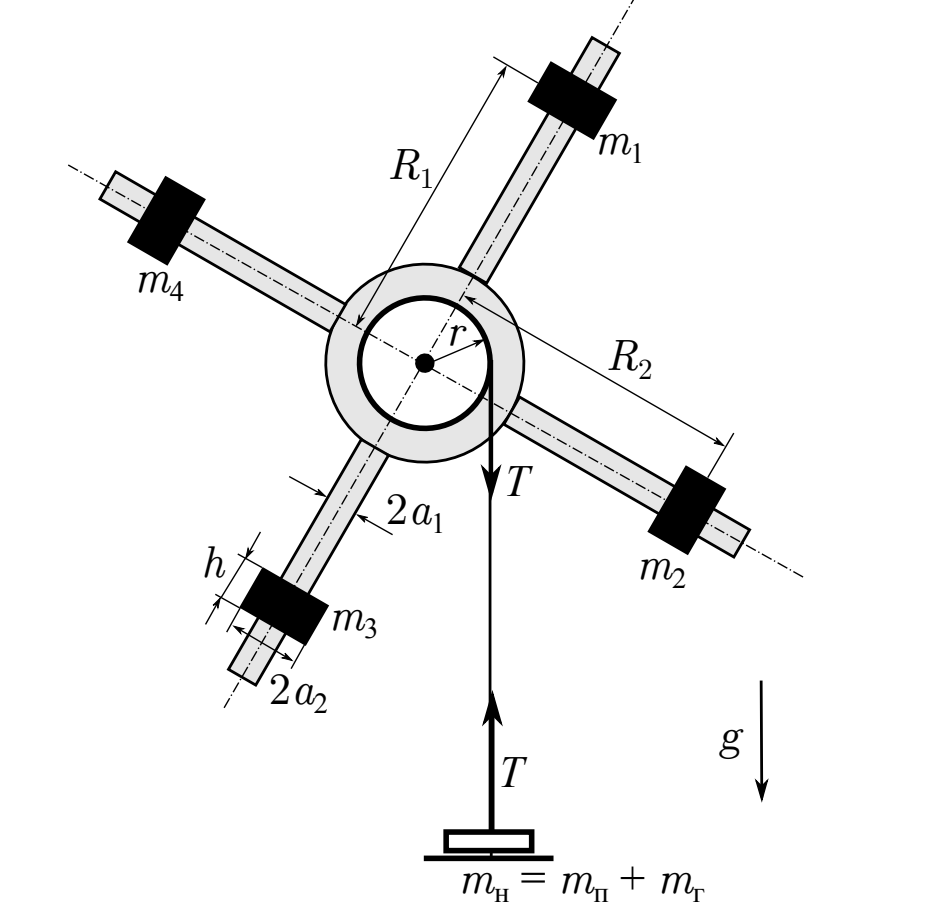
\includegraphics[scale=0.6]{picks/scheme_1.png} \\
    \textit{\textcolor[HTML]{000000}{Рис. 1. Крестообразный маятник Обербека}}
\end{center}
    
	\headheight = 0.5cm %размер верхнего колонтитула
	\headsep = 1.2cm %отступ после верхнего колонтитула
	
	\section{\Large Формулы: }


\newcommand{\formula}[2]{
\noindent#1\\[0.2cm]
    \begin{equation}
        #2
    \end{equation}
}

\newcommand{\mth}[1]{
\begin{math}
    #1
\end{math}
}
\newcommand{\ruB}[1]{
    _{\text{#1}}
}

\formula{Основное уравнение вращательного движения тела вокруг закреплённой оси:}{I\ddot{\phi} = M}

\subsection{\large Вывод уравнения движения маятника:}

\formula{Момент силы натяжения нити:}{M\ruB{н} = m\ruB{н}r\left(g - \beta r\right)}

\formula{Вращению маятника препятствует момент силы трения в оси \mth{M\ruB{тр}}.
Таким образом, с учетом (2) уравнение (1) может быть записано как:}{\left( I + m\ruB{н}r^2\right)\beta = m\ruB{н}gr - M\ruB{тр}}

\noindentПоскольку в опытах, как правило, \mth{m\ruB{н}r^2 \ll I}, и соответственно \mth{M\ruB{н} \approx m\ruB{н}gr}. Если трение мало,\\ \mth{ M\ruB{тр} \ll m\ruB{н}gr}, то маятник будет раскручиваться с постоянным угловым ускорением \mth{\beta_0 \approx m\ruB{н}gr/I}\\[0.4cm]

\formula{Зависимость момента силы трения от нагрузки на маятник и скорости его вращения не известна, но в общем случае есть как составляющая, пропорциональная угловой скорости \mth{\omega}, так и составляющая, пропорциональная силе реакции в оси N. Учитывая, что сила реакции уравновешеннего маятника равна \mth{N = m\ruB{м}g + T \approx \left( m\ruB{м} + m\ruB{н} \right)g \approx m\ruB{н}g}, где \mth{m\ruB{м}} - масса маятника (как правило, \mth{m\ruB{м} \gg m\ruB{н}}, можно записать:
}{
M\ruB{тр} \simeq \left(1 + \frac{m\ruB{н}}{m\ruB{м}}\right)M_0 + \mu\omega \approx M_0 + \mu\omega}

\noindentГде \mth{M_0} - момент сил трения для покоящегося маятника при нулевой массе подвеса (минимальное значение силы трения), \mth{\mu}— некоторый коэффициент, отвечающий за вязкое трение.\\[0.2]

\subsection{\largeМетодика эксперемента}\\[0.2]

Если верны высказанные выше соображения о величине силы трения, из (3) и (4) следует, что угловое ускорение должно быть линейной функцией угловой скорости:\mth{\beta(\omega) = \beta_0 + k\omega}.c В таком случае, определив по экспериментальным данным (с помощью расчётной программы) коэффициенты прямой, можно найти начальное угловое ускорение \mth{\beta_0} , значение которого и используется при проверке основного соотношения (3) при различных параметрах системы (\mth{m\ruB{н}, I, r}).\\[0.2]

\formula{Момент нерции системы расчитывается по теореме Гюйгенса-Штейнера:}{
I = I_0 + \displaystyle\sum_{i=1}^{4} \left( I_i + m_{i}R_{i}^2\right),}

\noindentгде \mth{I_0} - момент инерции системы без грузов,

\formula{}{
I_i = \frac{1}{12}m_{i}h^2 + \frac{1}{4}m_{i}\left(a_{1}^2 + a_{2}^2 \right)}\\[0.1]

\noindent- момент инерции i-го груза (грузы имеют форму полых цилиндров) относительно оси, проходящей через его центр масс (перпендикулярно плоскости рис. 1). Где \mth{a_1} и \mth{a_2} - внутренний и внешний радиус цилиндров, h - образующая цилиндров.
\newpage
	
\section{\Large Ход работы:}

\subsection{Балансировка:}
\noindentУстановил грузы \mth{m_i} на  некотором (среднем) расстоянии от оси шкива, так чтобы маятник оказался в положении безразличного равновесия. Провел балансировку, незначительно изменяя положения грузов.\\[0.2]

\noindentПоложения грузов \mth{R_i}:\\[0.1cm]
\mth{R_1 = 11,88\text{\qquad cм}}\\
\mth{R_2 = 12,46\text{\qquad см}}\\
\mth{R_3 = 12,15\text{\qquad см}}\\
\mth{R_4 = 11,85\text{\qquad см}}\\

\noindentМассы грузов \mth{R_i}:\\[0.1cm]
\mth{m_1 = 146,6\text{\qquad г}}\\
\mth{m_2 = 146,3\text{\qquad г}}\\
\mth{m_3 = 146,3\text{\qquad г}}\\
\mth{m_4 = 152,7\text{\qquad г}}\\


\subsection{Измерение момента силы трения покоя:}

\noindentНамотал на меньший из шкивов нить в один слой и подвесил на ней к маятнику пустую платформу. Нагрузил платформу так, чтобы маятник пришел в движение.\\[0.2]

\noindentГраничное значение момента силы трения покоя \mth{M_0 = 0,0075 Hm}\\[0.2]

\subsection{Ознакомление с "Kinematic":}

\noindent Включил компьютер и запустил расчетно-измерительную программу «Kinematic». Ознакомился с краткой инструкцией по работе с
программой.

\subsection{Нахождение коэффициентов для зависимости $\beta = \beta_0 + k\omega$:}

\noindentНамотал нить в один слой на больший из шкивов и поместил перегрузок (\mth{m\ruB{г}} = 27,2г) на платформу. Провел опыт: с помощью программы измерил зависимость угла поворота маятника от времени в процессе опускания платформы из верхнего в нижнее положение.\\[0.2]

\noindentПолученные значения:\\[0.2cm]
$
\begin{matrix}
    \beta_0 & = &  0,521  &\frac{\text{рад}}{\text{с}^2}\\
    k & = &  -0,0225  &\frac{\text{рад}}{\text{с}}\\
    {\big\sigma_{\beta_0}} & = &  0,006  &\frac{\text{рад}}{\text{с}^2}\\
    {\big\sigma_k} & = &  0,006  &\frac{\text{рад}}{\text{с}}\\
\end{matrix}
$

\newpage

\subsection{Оценка случайной погрешности:}
Провел серию эксперементов для фиксированных значений массы и момента инерции маятника, чтобы вычислить случайную ошибку  \mth{\sigma_\beta}. Значения для эксперементов приведены в таблице 1.\\[0.2]

\begin{table}[h!]
	\begin{center}
		\caption*{\color[HTML]{000000}Таблица 1: значения для вычисления случайной погрешности}
		\begin{tabular}{|P{3.8cm}|P{1.3cm}|P{1.3cm}|P{1.3cm}|P{1.3cm}|P{1.3cm}|P{1.3cm}|}
			\hline
            Номер эксперемента&1&2&3&4&5&6\\%9
            \hline
            $\beta_0,  \frac{\text{рад}}{\text{с}^2}$ &0,513&0,509&0,510&0,511&0,511&0,513\\
            \hline
            $k, \frac{\text{рад}}{\text{с}}$ &-0,026&-0,021&-0,021&-0,026&-0,021&-0,025\\
			\hline
		\end{tabular}
	\end{center}
\end{table}

Тогда сулчайная ошибка \mth{\sigma_\beta = \qquad\frac{\text{рад}}{\text{с}^2}}

\subsection{Опыты с разными перегрузками ${m\ruB{г}}$}

\noindentПровел эксперемент п. 2.4. для 8 различных значений момента силы натяжения нити, используя перегрузки \mth{m\ruB{г}} в диапазоне от 20 до 200 г на разных шкивах. Результаты эксперементов приведены в таблице 2 и таблице 3.

\begin{table}[h!]
	\begin{center}
		\caption*{\color[HTML]{000000}Таблица 3: значения для большого шкива}
		\begin{tabular}{|P{3.8cm}|P{1.3cm}|P{1.3cm}|P{1.3cm}|P{1.3cm}|P{1.3cm}|P{1.3cm}|P{1.3cm}|P{1.3cm}|}
			\hline
            Номер эксперемента&1&2&3&4&5&6&7&8\\%9
            \hline
            ${m\ruB{г}}, \text{кг}$&0,043&0,068&0,079&0,116&0,143&0,168&0,180&0,216\\
            \hline
            ${M\ruB{г}}, H\text{м}$&0,0093&0,0178&0,022&0,034&0,044&0,052&0,056&0,069\\
            \hline
            $\beta_0, \frac{\text{рад}}{\text{с}^2}$&0,519&0,819&0,962&1,436&1,768&2,055&2,219&2,648\\
            \hline
            $k, \frac{\text{рад}}{\text{с}}$&-0,026&-0,023&-0,024&-0,025&-0,025&-0.026&-0,026&-0,028\\
			\hline
            $\sigma_{\beta_0}, \frac{\text{рад}}{\text{с}^2}$&0,003&0,003&0,008&0,005&0,007&0,009&0,008&0,007\\
            \hline
            $\sigma_{k}, \frac{\text{рад}}{\text{с}}$&0,003&0,004&0,003&0,003&0,003&0,003&0,003&0,004\\
			\hline
		\end{tabular}
	\end{center}
\end{table}

\newpage

\subsection{Исследование зависимости углового ускорения от момента инерции системы:\\[0.2]}

Исследую зависимость углового ускорения от момента инерции системы. Для этого при значении массы перегрузка \mth{m\ruB{г} = 0,116 \text{кг}} проведу измерения при 5 различных значениях расстояния от оси системы до центров масс грузов. Результаты эксперементов предоставлены в таблице 3.\\[0.2cm]


\begin{table}[h!]
	\begin{center}
		\caption*{\color[HTML]{000000}Таблица 3: Исследование зависимости углового ускорения от момента инерции системы}
		\begin{tabular}{|P{3.8cm}|P{1.3cm}|P{1.3cm}|P{1.3cm}|P{1.3cm}|P{1.3cm}|}
			\hline
            Номер эксперемента&1&2&3&4&5\\
            \hline
            ${R}, \text{м}$&0,064&0,089&0,129&0,164&0,054\\
            \hline
            ${M\ruB{г}}, \text{Нм}$&0,348&0,348&0,348&0,348&0,348\\
            \hline
            $\beta_0, \frac{\text{рад}}{\text{с}^2}$&2,500&2,044&1,228&0,950&2,698\\
            \hline
            $k, \frac{\text{рад}}{\text{с}}$ &-0,042&-0,033&-0,022&-0,018&-0,0487\\
			\hline
            $\sigma_{\beta_0}, \frac{\text{рад}}{\text{с}^2}$&0,003&0,006&0,005&0,006&0,013\\
            \hline
            $\sigma_{k}, \frac{\text{рад}}{\text{с}}$&0,003&0,006&0,002&0,003&0,005\\
			\hline
		\end{tabular}
	\end{center}
\end{table}

\subsection{Измерение $I_0$:}

\noindent Снял грузы и провел серию эксперементов чтобы рассчитать $I_0$.\\[0.2]

\noindentРезультаты эксперементов предоставлены в таблице 4.\\[0.2cm]

\begin{table}[h!]
	\begin{center}
		\caption*{\color[HTML]{000000}Таблица 5: Измерение $I_0$}
		\begin{tabular}{|P{3.8cm}|P{1.3cm}|P{1.3cm}|P{1.3cm}|P{1.3cm}|P{1.3cm}|}
			\hline
            Номер эксперемента&1&2&3&4&5\\
            \hline
            $\beta_0, \frac{\text{рад}}{\text{с}^2}$&3,398&3,472&3,402&3,474&3,478\\
            \hline
            $k, \frac{\text{рад}}{\text{с}}$ &-0,051&-0,058&-0,051&-0,057&-0,051\\
            \hline
            $I_{0}, \text{кгм}^2$ &&&&&\\
			\hline
            $\sigma_{\beta_0}, \frac{\text{рад}}{\text{с}^2}$&0,008&0,016&0,012&0,018&0,014\\
            \hline
            $\sigma_{k}, \frac{\text{рад}}{\text{с}}$&0,003&0,006&0,004&0,006&0,004\\
			\hline
		\end{tabular}
	\end{center}
\end{table}

\end{document}
